\documentclass[aps, pre, preprint, groupedaddress, superscriptaddress, showkeys, showpacs] {revtex4-1}

\usepackage{amsmath}
\usepackage{mathtools}
\usepackage{amssymb}
\usepackage{amsfonts}
\usepackage{graphicx}
\usepackage{epstopdf}

% For the debug usage only
\usepackage{color}

\DeclarePairedDelimiter\bra{\langle}{\rvert}
\DeclarePairedDelimiter\ket{\lvert}{\rangle}

% Remove ugly line above reverences
\def\bibsection{\section*{\refname}}

% For the debug usage only
\newcommand{\red}{\color{red}}
\newcommand{\blue}{\color{blue}}

\begin{document}

\title{{Exciton-polariton Josephson junctions at finite temperatures}}

\author{M. E. Lebedev}
\affiliation{ITMO University, St. Petersburg 197101, Russia}

\author{D. A. Dolinina}
\affiliation{ITMO University, St. Petersburg 197101, Russia}

\author{S. M. Arakelian}
\affiliation{Vladimir State University named after A. G. and N. G. Stoletovs, Gorkii Street 87, Vladimir, Russia}

\author{Tien-Chang Lu}
\affiliation{Department of Photonics, National Chiao Tung University, Hsinchu 300, Taiwan}

\author{A. V. Kavokin}
\affiliation{Spin Optics Laboratory, St. Petersburg State University, Ul’anovskaya, Peterhof, St. Petersburg 198504, Russia}
\affiliation{School of Physics and Astronomy, University of Southampton, SO17 1BJ Southampton, United Kingdom}

\author{A. P. Alodjants}
\email{alexander\_ap@list.ru}
\affiliation{ITMO University, St. Petersburg 197101, Russia}
\affiliation{Vladimir State University named after A. G. and N. G. Stoletovs, Gorkii Street 87, Vladimir, Russia}

\date{\today}

\begin{abstract}
We consider the problem of achievement of quantum regime for relative phase of trapped in W -- potential low branch exciton polariton condensates taken at finite temperatures and finite polariton lifetime.
Non-standard Bose-Hubbard model for an exciton polariton Josephson junction (EPJJ) that is characterised by complex potential energy landscapes (PEL) consisting of sets of barriers and wells is proposed.
We have shown that the classical (thermal) activation and quantum tunneling for the phase represent two regimes depending on temperature, polariton condensate density and distance between the junctions.
The transition between these two regimes exhibits universal features of first or second order phase transition (PT) depending on the PEL for the relative phase of two polariton condensates.
In the presence of dissipation quantum system exhibits the non-equilibrium PT from quantum {\blue (where tunneling is possible)} to classical regime, where the tunelling is efficient and where it is suppressed, respectively.
The obtained results are discussed in details in the framework of the quantum annealing problem with exciton polariton condensates.   
 
\end{abstract}

\pacs{\dots}
\keywords{\dots}

\maketitle

\newcommand{\sn}{\textrm{sn}}
\newcommand{\cn}{\textrm{cn}}
\newcommand{\dn}{\textrm{dn}}
\newcommand{\sd}{\textrm{sd}}
\newcommand{\cd}{\textrm{cd}}
\newcommand{\nd}{\textrm{nd}}
\newcommand{\am}{\textrm{am}}

\section{Introduction \label{sec:introduction}}

In the last decade investigations of exciton polariton Bose-Einstein condensates (BEC) in various type of semiconductor microstructures represented an important mainstream of current photonic and semiconductor studies, see e.g. \cite{Sanvitto, Guillet}.
The microcavity exciton polaritons are bosonic quasiparticles representing  admixtures of the quantized cavity mode and quantum well excitons.
Semiconductor microcavities are promising for various optoelectronic applications where the quantum  matter-field interface plays crucial role.
In particular, it is worth to mention demonstrations of a polariton laser with electrical injection pump \cite{Bhattacharya,Schneider}, amplifiers \cite{Niemietz}, switches \cite{Amo_2010}, transistors \cite{Ballarini}, polariton circuits and optical logic elements \cite{Sturm,Liew}.
Although exciton polariton condensates exhibit Bose-Einstein statistics  above the lasing threshold under the phase transition (PT) condition and macroscopic occupation of the ground state at certain pumping rate that is less than for convenient lasers, they are not in true thermodynamic equilibrium state \cite{Byrnes_2014,Sun}. Non-equilibrium features of exciton polariton condensates play important role in various manifestations of their collective (many body) states such as superfluidity \cite{Carusotto_2013,Amo_2009}, quantized vortices \cite{Lagoudakis_2008,Lagoudakis_2009}, soliton formation \cite{Sich}, Josephson oscillations and macroscopic self-trapping \cite{Abbarchi,Lagoudakis_2010}.

Recently Yongbao Sun et al, in Ref. \cite{Snoke_2017} reported observation of a quasi-equilibrium low branch exciton polariton condensate in a high Q-factor microcavity possessing very a comparatively very long photon lifetime of $135ps$. Notably, exciton polaritons with long lifetime are promising candidates for quantum technologies, cf. \cite{Demirchyan}. However, since exciton polariton BEC's in present experiments are observed at high enough (up to the room) temperatures the quantum properties of such a states should be examined even at full thermal equilibrium. 
    
The problem of distinguishability of statistically classical and quantum regimes for exciton polariton condensates behavior is very actual for their practical applications and especially for their possible applications in quantum information technologies, see e.g. \cite{Dominici}.
Fast switching properties (the typical switching time of a few picoseconds), relatively strong nonlinear response and flexibility to external optical and/or electrical pump, spin degrees of freedom made microcavity polaritons potentially very promising for quantum computation and quantum information processing objectives, see, e.g. \cite{Demirchyan,Pagel,Kyriienko,Solnyshkov_2015, Dominici}.

Especially it is important to stress here quantum annealing problem physically based on the searching algorithm for the global minimum of a potential energy landscape (PEL) consisting of a set of barriers and wells, see e.g.  \cite{Santoro, Das}. In purely classical  (thermal) regime the {bosonic quasipartcles cross barriers stochastically} at finite temperature with the help of thermal activation process if the thermal energy is enough. Contrary, in a quantum limit the same system undergoes quantum tunneling through the barrier. Obviously, the shape of the barrier plays an essential role in this case, cf. \cite{Das, Lewenstein}. It has been shown recently in \cite{Lewenstein} that the annealing algorithm relies in general case on combination of thermal annealing and quantum tunneling. The     
collective (bosonic) character of polariton condensation could be used for the acceleration of the physical implementation of the search algorithm \cite{Yan}.  
  
In the paper we consider a generic problem of quantum-classical phase transition (PT) with exciton polariton condensates formed in a semiconductor microcavity in the presence of Josephson effect, cf. \cite{Chudnovsky_1997,Aleiner, Shelykh_2008, Borgh_2010}. To be more specific we examine simply a two junction model.
 
In general this problem relates to dissipative tunneling problem or, tunneling at finite (non-zero) temperatures, cf. \cite{Caldeira, Larkin, Riseborough}.
Traditionally,  studies in this field are limited by consideration of superconductor devices \cite{Ankerhold} where macroscopic quantum tunneling phenomena plays essential role.
In particular, it is worth to mention here the Schr\"odinger cat state formation \cite{Leggett} and the 	design of quantum gates with superconductor qubits for quantum computing where a macroscopic quantum coherence for the phase is important \cite{Makhlin}.
Recently the problem of quantum tunneling and quantum-classical PT problem have been examined for other two-level (spin) systems, like atomic BEC's \cite{Zhang}, and small ferromagnetic particles, \cite{Owerre}.
  
In the paper we consider an \textit{extended model} for exciton polariton Josephson junctions (EPJJs) that relates to so-called non-standard Bose-Hubbard models (see \cite{Dutta} and references therein) when energy of polariton-polariton scattering contributes into the tunneling parameter matrix elements, cf. \cite{Aleiner, Shelykh_2008, Borgh_2010, Solnyshkov_2008, Sarchi}.
In particularly, we pay attention to temperature dependent quantum critical phenomena occurring in the presence of macroscopic tunneling.
We aimed at formulating necessary criteria to obtain quantum phase regimes with trapped exciton polaritons suitable for realisation of quantum annealing purposes and creation of exciton polariton qubit gates.

This paper is arranged as follows.
In Sec. \ref{sec:quantum_phase} we introduce the quantum phase model for extended model of EPJJ of the coupled condensates and discuss various regimes for it at zero temperature and infinite exciton polariton lifetime. Section \ref{sec:quantum_classical} establishes  results obtained for quantum-classical PT problem and considered for quantum phase  at finite temperatures.  The influence of non-equilibrium effects with microcavity exciton polaritons possessing finite lifetime is discussed in \ref{sec:non-equilibrium}.      
In Conclusion we summarize the results obtained.
In Appendix \ref{sec:model} we explain in details  extended model of EPJJ within the tight-binding approach. 
\section{The Quantum Phase Model \label{sec:quantum_phase}}

We start with the Hamiltonain 
%
\begin{equation}
\hat{H} = \alpha \hat{S}_z^2 + \beta \hat{S}_x^2 - B \hat{S}_x.
\label{eq:hamiltonian_spin}
\end{equation}
that characterize weakly interacting exciton polariton condensate Josephson junction device in terms of pseudo-spin operators $\hat{S}_i$, $i=x,y,z$.
The parameters $\alpha$, $\beta$ and $B$ reflect  Josephson junction properties and determined in Appendix \ref{sec:model}. 
Here we propose quantum mechanical approach to the EPJJ  phase recasting pseudo-spin operators in  (\ref{eq:hamiltonian_spin}) through the differential representation defined as
% 
\begin{subequations}
\begin{align}
\hat{S}_x = & s \cos{\phi} - \sin{\phi} \dfrac{d}{d \phi}, \\
\quad \hat{S}_y = & s \sin{\phi} + \cos{\phi} \dfrac{d}{d \phi}, \\
\hat{S}_z = & -i\dfrac{d}{d \phi}
\end{align}
\label{eq:pseudo_spin_diff}
\end{subequations}
%
where  $\phi$ is the phase variable.
The operators determined in Eq. (\ref{eq:pseudo_spin_diff}) in \eqref{eq:hamiltonian_spin}
 obey familiar $SU(2)$ algebra commutation relations $[\hat{S}_i, \hat{S}_j] = i\epsilon_{ijk}\hat{S}_k,  i,j,k=x,y,z$.
After straitforward calculations from (\ref{eq:hamiltonian_spin}) one can obtain
%
\begin{equation}
\begin{array}{lcl}
H & = & -(\alpha - \beta \sin^2 \phi) \dfrac{d^2}{d \phi^2} - (\beta(s-\dfrac{1}{2})\sin{2\phi} - B\sin{\phi}) \dfrac{d}{d \phi} \\
&& - Bs \cos \phi - \beta s^2 \sin^2 \phi - \beta s \cos^2 \phi.
\end{array}
\label{eq:hamiltinian_s}
\end{equation}
%
We also assume macroscopically large particle number, i.e. the $s = N/2 >> 1$ is C - number. Using (\ref{eq:hamiltinian_s})  for Schrodinger equation we obtain   
%
\begin{equation}
\begin{array}{l}
(\alpha - \beta \sin^2 \phi) \dfrac{d^2 \Phi}{d \phi^2} + (\beta s\sin{2\phi}-B\sin{\phi})) \dfrac{d \Phi}{d \phi} \\
+ (E + B s \cos \phi + \beta s^2 \sin^2 \phi) \Phi = 0,
\end{array}
\label{eq:schrodinger}
\end{equation}
%
where $\Phi \equiv \Phi(\phi)$ is unknown $2\pi$-periodic wavefunction that characterizes quantum phase properties, cf. \cite{Anglin}.
%ng that Eqs. (\ref{eq:hamiltinian_s}), (\ref{eq:schrodinger}) can be obtained by applying so-called phase-state representation, {\red cf. [  ]}.
%
%\begin{equation}
%\ket{\psi} = \dfrac{1}{2 \pi} \int_{-\infty}^{+\infty} d \phi \Phi(\phi) \ket{\phi}
%\end{equation}
%
%where
%
%\begin{equation}
%\ket{\phi} = \dfrac{1}{\sqrt{N!}} \Big[ e^{i\phi/2} \psi_1^\dagger + e^{-i \phi/2} \psi_2^\dag \Big]^N \ket{0}_1\ket{0}
%\end{equation}
%
%is macroscopic coherent spin-state (macroscopic qubit state) that plays important role in current quantum information protocols operating with $N$-particle condensates, cf. \cite{Byrnes_2012}.
It is possible to eliminate the term with first derivative in Eq. (\ref{eq:schrodinger}) applying the transformation
%
\begin{equation}
\Phi(\phi) = \Psi(z) \exp \Big( s \ln \dn{z} - \dfrac{\Lambda s}{2 \sqrt{\lambda (1 - \lambda)}} \arctan \Big( \sqrt{\dfrac{\lambda}{1 - \lambda}} \cn{z} \Big) \Big),
\label{eq:transformation_of_phi}
\end{equation}
%
where $z = \int \limits_0^\phi \dfrac{d \xi}{\sqrt{1 - \lambda \sin^2 \xi}} = F(\phi, \lambda)$ is new phase variable; $F(\phi, \lambda)$ is incomplete elliptic integral of the first kind.
In (\ref{eq:transformation_of_phi}) we have introduced dimension-less parameters $\Lambda = \dfrac{G}{\alpha s}$, $\lambda = \dfrac{\beta}{\alpha}$ playing crucial role for our model.
Inserting (\ref{eq:transformation_of_phi}) into (\ref{eq:schrodinger}) we arrive to Schr\"odinger-like equation
% 
\begin{equation}
\alpha \frac{d^2\Psi}{dz^2} + (E - V(z))\Psi = 0
\label{eq:schrodinger_usual}
\end{equation}
%
characterizing quantum particle with the ``mass''  $m = \dfrac{\hbar^2}{2 \alpha}$ and energy $E$, that moves in the potential $V(z) = \alpha s^2 V_0(z)$ with
%
\begin{equation}
V_0(z) = \frac{ (\frac{1}{4} \Lambda^2 - \lambda (1 - \lambda)) \sn^2{z} - \Lambda \cn{z}}{\dn^2{z}}.
\label{eq:potential}
\end{equation}
%

The dependences of trapping potential $V_0(z)$ on phase variable $z$ are shown in Fig. \ref{phase_potential}. The period of the functions is  $4K(\lambda)$.
The dependence of the $\lambda$ parameter on normalized half of inter-well distance $\dfrac{x_0}{a}$ can be estimated as $\lambda = 0.5 \Big( \exp \Big[ \dfrac{2 x_0^2}{a^2} \Big] - 1 \Big)^{-1}$. The results known for quantum phase mesoscopic Josephson junction model can be recovered from (\ref{eq:hamiltonian_spin}), (\ref{eq:potential}) at $\lambda = 0$ and shown by red curves in  Fig.\ref{phase_potential}. This limit corresponds to  infinitely large inter-well distances, with $x_0 \to \infty$.
On the other hand, $\lambda$ -- parameter grows rapidly at $\dfrac{x_0}{a} \ll 1$.
Obviously, in this limit our EPJJ model that based on assumption of relatively weak coupling between the wells breaks down.

Below we are focusing on $\lambda$ -- parameters which belong to segment of $0 < \lambda < 1$ and might be obtained at moderate values of $\dfrac{x_0}{a}$ which are $\dfrac{x_0}{a} \geq 0.45$. 

%
\begin{figure}[ht]
\begin{center}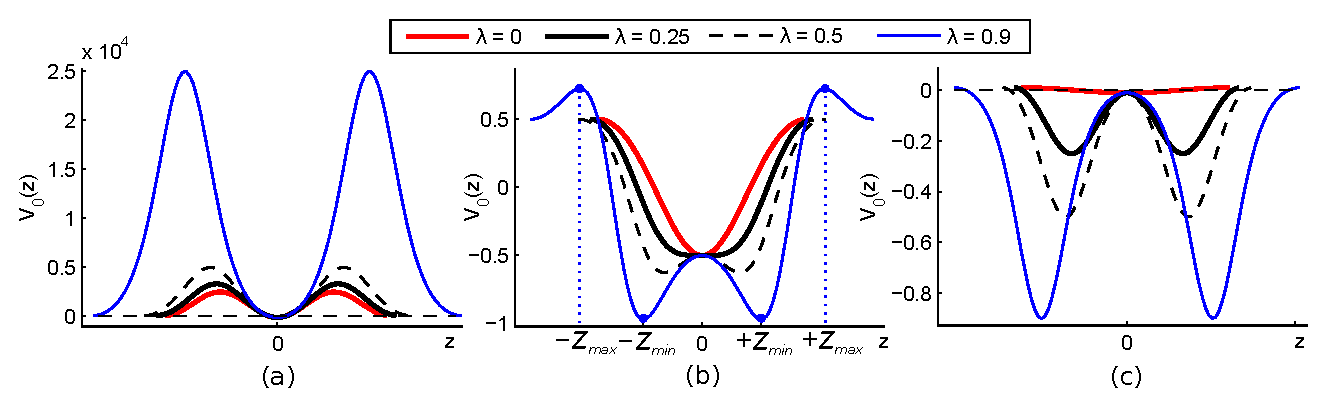
\includegraphics[width=1\linewidth]{pic/potentials.eps}
\end{center}
\caption{
Effective dimension-less potential $V_0(z)$ for (a) $\Lambda = 100$, (b) $\Lambda = 0.5$ , and (c) $\Lambda = 0.01$ as a function of elliptic integral phase coordinate $z$.
Points $\pm z_{min}$ and $\pm z_{max}$ in (b) relay to global minima and maxima of the potential, correspondingly, occurring with periodicity $4K(\lambda)$. \label{phase_potential}}
\end{figure}
%

Analysis of the quantum phase can be performed  in three domains determined by vital $\Lambda$--parameter values, cf. \cite{Anglin}.

\textit{Rabi regime} $\Lambda \gg 1$. In this limit the trapping potential reads $V_R(z) = \dfrac{1}{4} \Lambda^2 \sd^2{z}$.
Physically, for any value of $\lambda$ -- parameter taken from the domain 0$<\lambda <1$ we can obtain (Rabi) oscillations for quantum phase.
In particular, small amplitude oscillations which are inherent to familiar Rabi regime can be achieved for negligable $\lambda$ --- see Fig. \ref{phase_potential}a and cf. \cite{Anglin}.

\textit{Fock regime} $\Lambda \ll 1/N^2$.
In purely quantum limit 
%the two mode system approaches by the state $\ket{\psi} \propto (\psi_1^\dag)^s (\psi_1^\dag)^s \ket{0}_1 \ket{0}_2$%
the phase wavefunction approaches $\Phi(\phi) \to (2\pi)^{-1/2}$.
In this regime, when inequality $\Lambda \ll \lambda < 1$ is holds, Eq.(\ref{eq:schrodinger_usual}) transforms into Mathieu equation that implies spectrum consisting from all Mathieu functions.

\textit{Josephson regime} $1/N^2\ll\Lambda <1$.
This regime represents intermediate case between Rabi and Fock limits --- see Fig. \ref{phase_potential}b.
The behavior of the phase depends on the ratio between parameters $\Lambda$ and $\lambda$.
If $\Lambda \ge 2\lambda$ the $V_0(z)$ posses only one minima at $z = 0$ and $V(0) = -\Lambda$. 
%Frequency of small amplitude ($z \ll 1$) oscillations %can be obtained from (\ref{eq:potential}) and looks like { \red $\omega_{0, quantum} = \frac{2 \alpha s}{\hbar} \sqrt{\frac{1}{4} \Lambda^2 - \frac{\Lambda}{2} (2\lambda - 1) - \lambda(1 - \lambda)}$ }.

In the other limit, for $\Lambda < 2 \lambda$, quantum "particle" is trapped at two minima of $V_0(z)$ that corresponds to $W$ -- like potential with coordinates $\cn{z_{min}} = \frac{\Lambda}{2 \lambda}$ and appearing for both of Josephson and Fock regimes, cf. Fig. \ref{phase_potential}b,c.  
The depth of the potential minima depends on the $\lambda$ parameter.
It is interesting to note that for $\Lambda > 2(1 - \lambda)$ potential $V_0(z)$ presumes local minimum at $\pm 2 K(\lambda)$, see Fig. 1b.

% $ce_0(z, q)$, $ce_1(z, q)$, $se_1(z, q)$, \dots, which are $2\pi$-periodic, and corresponding eigenvalues $a$ can be found using series expansions in powers of $q$.
%from (\ref{eq:potential}) one can obtain
%
%{\red

%
%\begin{equation}
%V_F(z) \simeq -\lambda (1 - \lambda) \sin^2{z},
%\end{equation}
%
%and our 
%transforms into Mathieu equation;
%
%\begin{equation}
%\frac{d^2 \Psi}{d z^2} + (a - 2q  \cos{2z}) \Psi = 0.
%\end{equation}
%
%where $a = E / \alpha + s^2 \lambda(1 - \lambda) / 2$, $q = s^2 \lambda (1 - \lambda)/ 4$.
%We recall our boundary condition: $\Psi(z + 2\pi) = \Psi(z)$.

%In another limit $\lambda \ll \Lambda$ 
%that might  be studied within Fock regime is relevant to condition . In this case from (\ref{eq:potential}) 
%we have $V_0(z) \simeq -\Lambda \cos{z}$.
%In fact, this limit that deals with negligible $\lambda$ reproduces results for convenient quantum phase model \cite{Anglin}.

\section{Annealing problem versus Quantum-classical PT's \label{sec:quantum_classical}}

In current experiments with exciton polaritons  the condensate is observed at finite and high enough temperatures \cite{Sanvitto,Guillet}.
In this section we find conditions when quantum approach to the phase problem for Josephson junction with coupled exciton polariton condensates is valid. This conditions, in fact, responsible for ability of our system to perform quantum annealing algorithm \cite{Das}.

To  be more specific we consider the tunneling in  effective $W$ -- like potential represented in Fig. \ref{phase_potential}b  inherent to  Josephson regime. We examine thermodynamically equilibrium (with infinitely large  exciton polariton lifetime) system of exciton polaritons at finite temperature $T$.  Noticing, that in  recent experiments  described in Ref. \cite{Snoke_2017} polariton lifetime attains  $275ps$ at resonance that seems to be enough to justify the quantum processes described below.

Transition between two stable states (say, between points $-z_{min}$ and $+z_{min}$ in Fig. \ref{phase_potential}b) can happen  either through the quantum tunneling or, in classical way, due to the thermal activation. 
Obviously, at high temperatures such as $k_{B}T\ge\Delta V$ ($\Delta V$ is height of the barrier between two states with minimum of potential energy) the particle jumps over the barrier governed by familiar thermoactivation (Arrhenius) escape rate $\Gamma \sim e^{-\Delta V /k_{B}T}$, cf. \cite{Larkin}. This process inherent to classical (thermal) annealing problem \cite{Das}. 

In the ``low temperature'' limit $k_{B}T\ll\Delta V$ particle undergoes quantum tunneling through the barrier with vanishing rate, that is important especially for quantum annealing scheme. 
%with the rate $\Gamma \sim e^{-B/\hbar}$, where $B$ is the instanton action.
%Now we elucidate conditions for their realization for exciton polariton Josephson junction problem. 

Our description is based on imaginary time path integral approach, cf. \cite{Ankerhold}.
The imaginary-time action obtained within WKB method approaches as $S(E) = \oint (\tfrac{1}{2} m \dot{z}^2 + V(z)) d \tau$.
%
%\begin{equation}
%S(E) = \oint (\tfrac{1}{2} m \dot{z}^2 + V(z)) d \tau.
%\label{eq:thermon_action_1}
%\end{equation}
%
The decay rate $\Gamma \sim e^{-S_{min}/\hbar}$ according to our approach can be expressed through the minimal value $S_{min}$ of the action.
The trajectories which are minimize the action $S_T$ satisfy to classical equation of motion $m \ddot{z} = \frac{d V}{dz}$ written for the thermon "particle" that  oscillates inside the inverted potential $-V(z)$. 
%
%\begin{equation}
%m \ddot{z} = \frac{d V}{dz}.
%\label{eq:thermon}
%\end{equation}
%
Periodic solutions of this equation satisfy
%
\begin{equation}
\tfrac{1}{2} m \dot{z}^2 = V(z) - E(\tau_p),
\label{eq:total_energy}
\end{equation}
%
where $\tau_p = \hbar / k_B T$ is a thermon period corresponding to the energy $E(\tau_p)$;
%
\begin{equation}
\tau_p(E) = \sqrt{2 m} \int_{z_1(E)}^{z_2(E)} \frac{dz}{\sqrt{V(z) - E}}.
\label{eq:thermon_period}
\end{equation}
%
In (\ref{eq:thermon_period}) the $z_{1,2}(E)$ are turning points, cf. Fig. \ref{phase_potential}b.
The Eqs.(\ref{eq:total_energy}),(\ref{eq:thermon_period}) taken at energy $E = 0$ and temperature $T = 0$ characterize instanton solution with infinite period.
Combining  equation for $S(E)$ 
%(\ref{eq:thermon_action_1}) 
with (\ref{eq:total_energy}) we arrive to 
%
\begin{equation}
S_T = 2 \sqrt{2 m} \int_{z_1(E)}^{z_2(E)} \sqrt{V(z) - E} ~dz + E \tau_p (E).
\label{eq:thermon_action_2}
\end{equation}
%

To determine thermodynamic properties of the system it is necessary to know small amplitude oscillations  at the bottom, $z=0$, of inverted potential $-V(z)$.
The action in this case reads: 
%
\begin{equation}
S_0 = \Delta V \tau_p (E).
\label{eq:thermal_action}
\end{equation}
%

Expansion of the potential $V(z)$ excluding constant value $V(0)$ gives:
%
\begin{equation}
\begin{array}{lcl}
V(z) & = & \alpha s^2 \Big[ \left( \frac{1}{4} \Lambda^2  - \frac{2\lambda - 1}{2} \Lambda - \lambda (1 - \lambda) \right) z^2 \\
&& + \left( \frac{2\lambda - 1}{12} \Lambda^2 - \frac{16\lambda^2 - 16\lambda + 1}{24} \Lambda - \frac{\lambda (1 - \lambda) (2\lambda - 1)}{3} \right) z^4 + o(z^4) \Big].
\end{array}
\label{eq:potential_teylor}
\end{equation}
%
In particularly, if the inverted potential $-V(z)$ has the form $z^2 - z^4$ the second order phase transition occurs.
If $-V(z)$ behaves as $z^2 + z^4$ first order phase transition take place.
Phase boundary between 1st and 2nd order phase transitions is determined by the relation
%
\begin{equation}
\Lambda = \frac{1 - 16\lambda + 16\lambda^2 + \sqrt{1 + 32\lambda - 32\lambda^2}}{4(2\lambda - 1)}.
\label{eq:order_border}
\end{equation}
%

We summarize our results in Fig. \ref{pic:phase_boundary_combined}. An insets demonstrate various type of  phase potentials $V_0(z)$ inherent to our EPJJ model. First order PT occurs for two type of potentials in the shaded region bounded by bold  (red) curve.  Second order PT's appear for potential landscapes taken from  dark area. 
%
\begin{figure}[ht]
\center{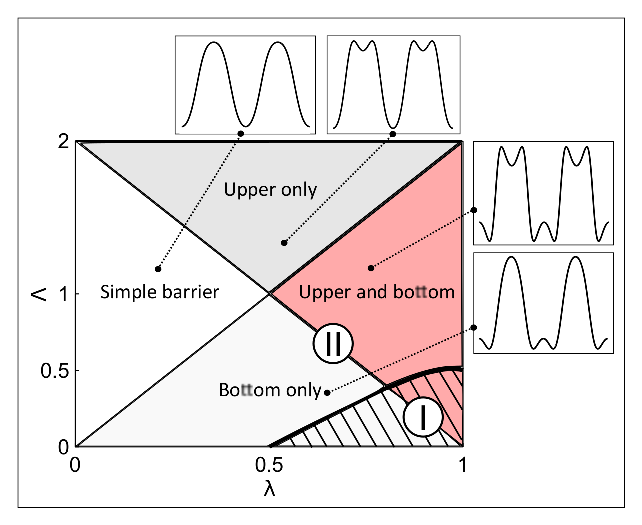
\includegraphics[width=0.5\linewidth]{pic/phase_transition_diagram_combined.eps}}
\caption{Diagram of the phase boundary for  1st- and 2nd-order  PT's in $\Lambda$,$\lambda$-parameters plane. The PEL's are shown in the windows. \label{pic:phase_boundary_combined}}
\end{figure}
%

The crossover temperature $T_{c}^{(2)} = \hbar \omega_0/ 2 \pi k_B$ of 2nd-order PT transition  is 
%
\begin{equation}
T_{c}^{(2)} = T_{0} \sqrt{\lambda (1 - \lambda) + (2 \lambda - 1) \tfrac{\Lambda}{2} - \tfrac{1}{4} \Lambda^2},
\label{eq:second_order}
\end{equation}
%
where  $\omega_0 = \frac{2 \alpha s}{\hbar} \sqrt{\lambda (1 - \lambda) + \tfrac{1}{2} (2 \lambda - 1) \Lambda - \tfrac{1}{4} \Lambda^2}$ is small oscillation frequency of thermon "particle" near the bottom of inverted potential,  $T_{0}=\alpha N / 2\pi k_B$ is some characteristic temperature that inherent to exciton polariton system.  The $T_{0}$  implies important time scale $\tau_0=2\pi\hbar/ \alpha N$ that can be understood as thermon particle ``lifetime''. Notably, as it is follows from (\ref{eq:second_order}) there is no barrier at $z = 0$ for $\Lambda \ge 2\lambda$ -- see white domain in Fig. \ref{pic:phase_boundary_combined}.

Figure \ref{pic:action_period}a displays 2nd-order PT from quantum (solid bold line of $S_T$) to thermal (classical) regimes --- dashed bold line of $S_0$.
The crossover occurs at the critical temperature $T_{c}^{(2)}$ where $S_T = S_0$ and {$E = E_0$}.
The inset demonstrate monotonic dependence of normalized thermon period $\tau_p/\tau_0$ on energy $E$ that is inherent to second-order phase transition.
Closest to the critical point with energy $E=E_0$ thermon undergoes small amplitude oscillations.  

%
\begin{figure}[ht]
\begin{minipage}[h]{0.49\linewidth}
\center{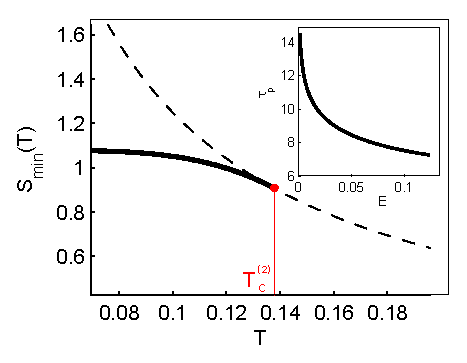
\includegraphics[width=1\linewidth]{pic/action_period_2nd_order_transition.eps} \\ (a)}
\end{minipage}
\hfill
\begin{minipage}[h]{0.49\linewidth}
\center{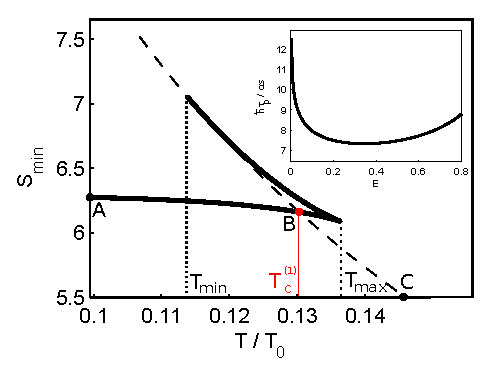
\includegraphics[width=1\linewidth]{pic/action_period_1st_order_transition.eps} \\ (b)}
\end{minipage}
\caption{Dependences of  minimal action $S_{min}$ (ABC-(blue) curve) taken in $s\hbar$ units as a function of normalized temperature $ T/T_{0}$ for (a) 2nd-order PT, $\lambda = 0.9$, $\Lambda = 0.1$; and, (b) 1st-order PT, $\lambda = 0.5$, $\Lambda = 0.5$; the solid (bold) line corresponds to the thermon action, $S_T$; the dashed line corresponds to the thermodynamic action, $S_0 = \hbar \Delta V / k_B T$, $S_{min} = \min \{S_0, S_T\}$. The inset shows dependences of normalized thermon period $\tau_p / \tau_0$ versus energy $E$ given in  $\alpha s^2$ units. 
\label{pic:action_period}}
\end{figure}
%
 
In Fig. \ref{pic:action_period}b we represent results exhibiting 1st-order PT inherent to narrow shadow domain in Fig.\ref{pic:phase_boundary_combined}.
It is clearly seen that the first derivative of $S_{min}$ is discontinuous in this case and the dependence of normalized thermon period  $\tau_p / \tau_0$ on energy $E$ is non-monotonic, see inset in Fig. \ref{pic:action_period}b.
The critical temperature $T_{c}^{(1)}$ belongs to the temperature domain $T_{min} < T_{c}^{(1)} < T_{max}$ and can be find out numerically by solving Eqs.(\ref{eq:thermon_period}) - (\ref{eq:thermal_action}) under the condition $S_T = S_0$.
 
Analytically critical temperature $T_{c}^{(1)}$ might be estimated from $T_{c}^{(1)} = \Delta V / B$, where $B$ is a instanton action that can be represented as $B = S(E_{min})$.
After some straightforward calculations for $B$ we obtain
%
\begin{equation}
\begin{array}{c}
B = S(E_{min}) = 2 s \hbar \left[ \ln \frac{2 \sqrt{\lambda} + \sqrt{4 \lambda^2 - \Lambda^2}}{2 \sqrt{\lambda} - \sqrt{4 \lambda^2 - \Lambda^2}} - \frac{\Lambda}{\sqrt{\lambda (1 - \lambda)}} \arctan \left( \frac{\sqrt{(1 - \lambda) (4 \lambda^2 - \Lambda^2)}}{\Lambda} \right) \right].
\end{array}
\label{eq:B_action}
\end{equation}
%

In experiments with exciton polaritons it is much more easier to manipulate by polariton density instead of the temperature, see e.g. \cite{Sanvitto,Guillet}.
For instance, the density of polariton gas can be changed by using external optical pump.
In Fig. \ref{pic:temperatures} we plot numerically calculated critical temperature of 1st and 2nd order PTs against $\Lambda$-parameter for experimentally accessible semiconductor Josephson junction samples.
Bold (green) line corresponds to analytical solution obtained with  Eq. (\ref{eq:B_action}).
Since the $\Lambda$-parameter is inversionally proportional to the density of exciton polariton gas (so-called blue shift) Fig. \ref{pic:temperatures} establishes important correspondence between critical temperatures discussed in the paper and relevant exciton polariton densities.
%
\begin{figure}[ht]
\center{\includegraphics[width=0.5\linewidth]{pic/phase_transition_temperatures.eps}}
\caption
{Dependence of normalized critical temperature $T_{c}/T_{0}$ as a function of parameter $\Lambda$. Bold (green) line corresponds to analytical solution for  $T_{c}^{(1)}$.     
\label{pic:temperatures}}
\end{figure}
%

Now let us consider decay of the upper state that is relevant to  upper minima located at $\pm 2K(\lambda)$ in Fig.\ref{phase_potential}b and exists for $\Lambda > 2(1 - \lambda)$. Physically this problem presumes tunneling through the barrier located at one of the point $z_{max} = \pm \cn^{-1} \left( -\frac{2(1 - \lambda)}{\Lambda} \right)$.
%small ocsillation frequency near the bottom $z_{max}$ of the inverted potential $\omega_0 = \frac{\alpha s}{\hbar} \sqrt{\frac{\Lambda^2}{1 - \lambda} - 4(1 - \lambda)}$.
By expanding the potential $V(z)$ near the vicinity of $z_{max}$ it is possible to show that only 2nd-order PT with temperature $T_{c}^{(2)} = (T_{0}/ 2) \sqrt{\frac{\Lambda^2}{1 - \lambda} - 4(1 - \lambda)}$ appear in this case.

Let us briefly discuss observation feasibility of quantum-classical PT for exciton polariton BEC's obtained in experiments. In particular, for experimentally accessible polariton interaction strength $\alpha N=0.6meV$, given for narrow-band semiconductor samples, the  $T_{0}$ is about $1.2K$ that is comparable with typical temperature of condensation, or, with temperature of Berezinsky-Kosterlitz-Thouless PT considered for dilute weakly interacting exciton polariton gas being at thermal equilibrium,cf. \cite{Sanvitto,Guillet}. Practically some enhancement of $T_{0}$ is possible by increasing of exciton polariton density and by improvement of experiment conditions, cf. \cite{Snoke_2017}.  
%
%\begin{equation}
%T_{c}^{(2)} = (T_{0}/ 2) %\sqrt{\frac{\Lambda^2}{1 - \lambda} - 4(1 - \lambda)}.
%\label{eq:second_order_2}
%\end{equation}
%


%With the aim of analytical determining of the phase transition order let's write the Taylor series for $V(z)$ near the vicinity of $z_{max}$.
%Expansion of the potential $V(z)$ excluding constant value $V(z_{max})$ gives:
%
%\begin{equation}
%V(\tilde{z}) = \alpha s^2 \Big[ -\tfrac{1}{4} \left( \tfrac{\Lambda^2}{1 - \lambda} - 4(1 - \lambda) \right) \tilde{z}^2 
%+ \tfrac{1}{2} \tfrac{\Lambda \sqrt{\Lambda^2 - 4(1 - \lambda)^2}}{\sqrt{1 - \lambda} \sqrt{\Lambda^2 + 4 \lambda (1 - \lambda}} \tilde{z}^3 + o(\tilde{z}^4) \Big],
%\label{eq:potential_teylor_2}
%\end{equation}
%
%where $\tilde{z} = z - z_{max}$.
%It follows from (\ref{eq:potential_teylor_2}) that $-V(\tilde{z})$ aways has the form $\tilde{z}^2 - \tilde{z}^3$, as $\Lambda > 0$, so in this case only second-order phase transition occurs.
% We plot typical behaviour of the $\tau(E)$, $S(T)$ and $T_{c}^{(2)}$ on Figs. \ref{pic:action_period_temperature_2}, and summarize our results on the Fig. \ref{pic:phase_boundary_combined}.
%
%\begin{figure}[ht]
%\begin{minipage}[h]{0.49\linewidth}
%\center{\includegraphics[width=\linewidth]{pic/action_period_2nd_order_transition_b2.eps} \\ (a)}
%\end{minipage}
%\hfill
%\begin{minipage}[h]{0.49\linewidth}
%\center{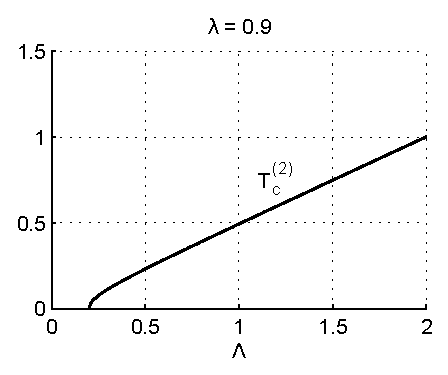
\includegraphics[width=\linewidth]{pic/phase_transition_temperatures_b2.eps} \\ (b)}
%\end{minipage}
%\caption{\dots \label{pic:action_period_temperature_2}}
%\end{figure}
%
\section{PT's in the presence of dissipation 
\label{sec:non-equilibrium}}

Let us now consider more realistic physical situation with EPJJ that valid for finite exciton polariton lifetime $\tau_{pol}$. Obviously, for finite $\tau_{pol}$  characteristic time $\tau_0$ that is responsible for quantum tunneling effects  should be shorter than typical time scales describing non-equilibrium processes with exciton polaritons. More precisely, in this case we require fulfillment of  inequality 
 \begin{equation}
 \tau_{0}\ll\tau_{pol}.
 \label{eq:lifetime}  
\end{equation}

In order,  characteristic  temperature $T_{0}=1.2K$ corresponds to thermon effective lifetime  $\tau_{0}=3.5ps$ for estimations given above. Here we examine situation when exciton polariton lifetime $\tau_{pol}$ is comparable with $\tau_{0}$. Namely  this situation is realized in most of current experiments with non-equilibrium exciton polariton condensates, see e.g. [   ].  

Below we consider the influence of the dissipation to  EPJJ quantum phase properties in adiabatic limit, cf. \cite{Sols}.
We start from GP equations obtained from  (\ref{eq:hamiltonian}) for mean fields $\psi_{1,2}=<\hat\psi_{1,2}>$  at $\Gamma = 0$ ($B = G$),  which reads as 
\begin{equation}
i \hbar \dot{\psi}_{1,2} = -i \kappa \psi_{1,2} + (A|\psi_{1,2}|^2 + 2C |\psi_{2,1}|^2) \psi_{1,2} - (B/2 - C \psi_{1,2}^* \psi_{2,1}) \psi_{2,1}. 
\label{eq:GP}
\end{equation}
In (\ref{eq:GP}) we introduced dissipation  term with $\kappa \simeq \hbar/\tau_{pol}$.
Defining new variables $\Psi_{1,2}$ by using  $\psi_{1,2} = \Psi_{1,2} \exp(-\kappa t / \hbar)$ for mean field pseudo-spin  parameters (\eqref{eq:pseudo_spin}) from {\ref{eq:GP}} we obtain
%
%
% 
\begin{equation}
\begin{array}{lcl}
\dot{S}_z & = &  2 \beta'(t) S_x S_y - S_y; \\
\dot{S}_x & = & -2 \alpha'(t) S_z S_y; \\
\dot{S}_y & = & 2(\alpha'(t) - \beta'(t)) S_z S_x + S_z.
\end{array}
\label{eq:pseudo-spin}
\end{equation}
%
Here we explore the dimensionless time $t' = t B / \hbar$.
This system describe dynamics of normalized mean field pseudo-spin parameters on the Bloch sphere with $S_x^2 + S_y^2 + S_z^2 = 1$.
Now set of Eqs.\ ({\ref{eq:pseudo-spin}}) looks similar to one taken for non-dissipative system but with time dependent parameters $\alpha'(t) = (1/ \Lambda) \exp(-2 \kappa t')$, $\beta'(t) = (\lambda / \Lambda) \exp(-2 \kappa t')$, cf.\cite{Sedov}. Without dissipation Eqs.\ ({\ref{eq:pseudo-spin}}) posses  bifurcation point $\lambda / \Lambda= 1 / 2$ that corresponds to solid black curve in Fig.1b. 

In Fig. \ref{pic:phase}a we plot phase difference $ \phi = \arctan(-S_y / S_x)$ between the junctions as a function of time.  Non-dissipative system has two different regimes depending on the values of  $\beta$ -- parameter, that is blue and red curves in the Fig. \ref{pic:phase}, respectively. Blue  curve is plotted under the condition $\beta' > 1/2$ and  corresponds to the existence of barrier for potential energy -- see Fig. \ref{pic:phase}b. Contrary,  red curve establishes phase properties below the threshold ($\beta' <1/2$) that corresponds to the absence of the barrier. 

In the presence of dissipation (solid black curve in Fig. \ref{pic:phase}a) phase of EPJJ starts from one of potential  minimum. It evolves adiabatically and then  crosses the critical value 1/2
due to decreasing of total number of particles. 
%It can be transformed to the equation on the phase difference $\phi$ and $S_z$ as follows
%
%\begin{equation}
%\begin{array}{lcl}
%\dot{S}_z & = & B \sqrt{1 - S_z^2} \sin \phi - 2 \beta(t) (1 - S_z^2) \sin \phi \cos \phi; \\[10pt]
%\dot{\phi} & = &  -2 \alpha(t) S_z + 2 %\beta(t) S_z \cos^2 \phi - \dfrac{B S_z \cos \phi}{\sqrt{1 - S_z^2}}.
%\end{array}
%\end{equation}
%
%We studied its dynamic numerically.
%
\begin{figure}[ht]
\center{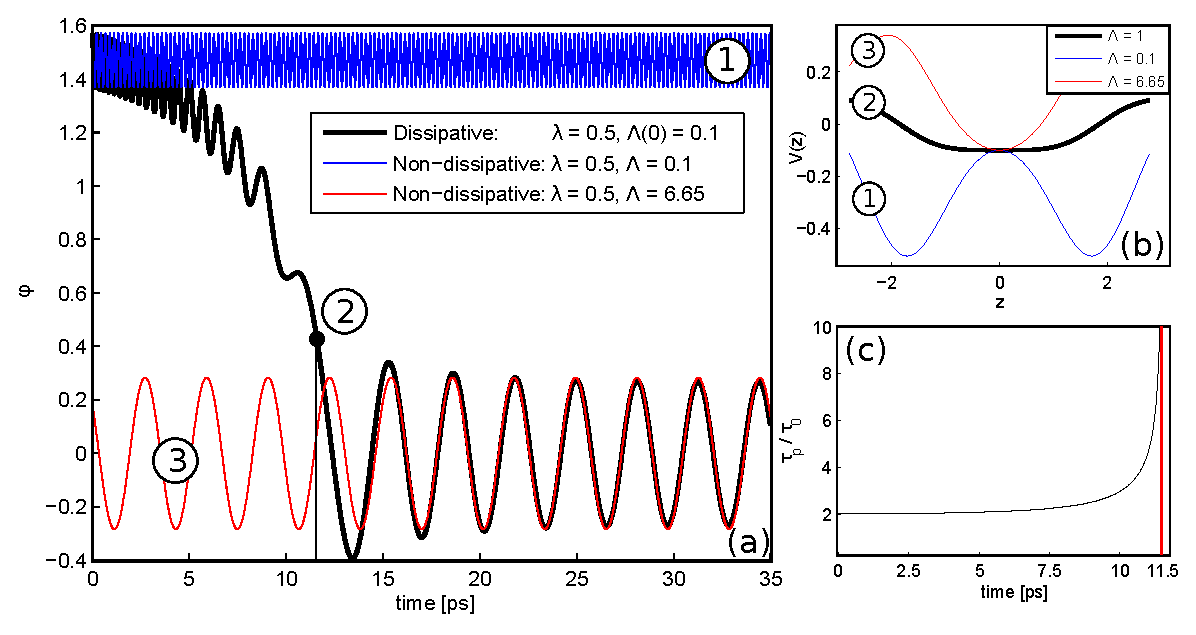
\includegraphics[width=\linewidth]{pic/phase_potential_dissipation.eps}}
\caption{(a) -- Normalized phase difference as a function of time; (b) -- effective potential vs phase parameter $z$ for red, black and blue curves respectively, and (c) -- reduced thermon period $\tau_{p} / \tau_0$ ($\tau_0 = \alpha s / \hbar$) vs time for $\kappa/\hbar = 0.1 THz$. 
Initial conditions are $S_z(0) = S_x(0) = 0$, $S_y(0) = 1$, and $\phi(0) = \pi / 2$, respectively.
\label{pic:phase}}
\end{figure}
%
%\begin{figure}[ht]
%\center{\includegraphics[width=0.5\linewidth]{pic/temperature_on_dissipation.eps}}
%\caption{Dependance of $T_c^{(2)}$ on $\kappa t$ for $\kappa / \hbar = 0.04 \cdot 10^{12}$ $1 / sec$, $B = 1$
%\label{pic:temperature_dissipation}}
%\end{figure}
%

The Fig. \ref{pic:phase}c exhibits suppression of critical temperature of phase transition $T_{c}^{(2)}$ that occurs at the timepoint $t_0=...$ for  $\tau_{pol} \sim \hbar/\kappa= 10 ps$.
 
Physically, behavior of the phase in the presence of dissipation showed in Fig. \ref{pic:phase} establishes non-equilibrium PT from regime where tunneling is possible to the regime where tunneling is suppressed. However, this regime happening at $t>t_0$ cannot be interpreted immediately as classical one.
  
Actually, adiabaticity condition reads, cf. {\cite{Sols}:
%
\begin{equation}
\dfrac{1}{\omega^2(t)} \Big| \dfrac{d \omega}{d t} \Big| \ll 1.
\end{equation}
%
where $\omega(t) = \sqrt{(B - 2\beta(t))(B - 2 \beta(t) + 2 \alpha(t))}$ is small amplitude oscillations slowly depending on time. 
%It allows us to reduce linear system to the harmonic oscillator equaiton with slowly evolving frequency:
%
%\begin{equation}
%\ddot{\phi} + \omega^2(t) \phi = 0,
%\end{equation}
%
The solution of the phase in this case can be given as 
\begin{equation}
\phi(\tau) \approx \dfrac{A}{\omega(\tau)} \cos (\omega(\tau) \tau),
\end{equation}
%
where $\tau$ is the time elapsed after the oscillation sets in, and $A$ is an amplitude of oscillations at the moment $\tau = 0$. At large enough times 
$\omega(t) \approx$ $B$  and permanent-like temporal oscillations for the Josephson junction phase $\phi$ are occurs, see Fig. 5a and cf.  [   ]. To determine quantum (or, classical) character of this oscillations quantum fluctuations should be examined.      


\section{Conclusion \label{sec:conclusion}}

Let us summarize the results obtained. In the paper we examine quantum phase properties for  extended EPJJs created with the help of coupled exciton polariton condensates taken at finite temperatures and finite exciton polariton lifetime. We have shown that  PEL with set of barriers and wells (various W--like potentials) can be achieved for our model  depending on the $\Lambda$ and $\lambda$ parameters which characterize condensate junctions. The W-shape potential at finite temperatures admits two regimes which are  purely quantum tunneling regime through the barrier or classical regime of thermal activation.   Transition (crossover) between this two limits exhibits universal features of 1st or 2nd order PTs which can be interpreted as PT between classical and quantum regimes. It is important that critical temperature of transition depends on some  characteristic temperature  parameter $T_{0}$ (see e.g. (\ref{eq:second_order})) that depends on polariton-polariton interaction length (so-called blue shift) $\alpha N$.  It is expected that  at the temperatures sufficiently higher than  $T_{0}$ the EPJJ device operates in classical way. 

The influence of dissipation effects to this picture is evident from our analysis. The observation of quantum tunneling processes become possible only within short time intervals when the dissipation cannot essentially affected to the system.
Otherwise, after some time interval dissipation leads to crossover in the phase dynamics and destroy the W--potential as whole, see Fig. \ref{pic:phase}. In this case permanent oscillations of Josephson junction phase occurs within adiabatic approach. To determine quantum either classical properties of this oscillations it is necessary to study fluctuations of the exciton polariton system beyond the semiclassical approach represented in Sec.\ref{sec:non-equilibrium}}. 
For moderate dissipation rates and at the temperatures (or relevant polariton gas densities) sufficiently below the temperature of $T_{0}$   the EPJJ device is  capable for various applications where quantum tunneling effect is crucial. 

First, it is quantum information processing and especially quantum annealing problem  with exciton polariton condensates that can be enhanced with the help of bosonic stimulation phenomena {\cite{Yan}. Notably the results obtained by us can be implemented  here in new way.  In order, quantum tunneling effect might be utilized  for design exciton polariton phase qubits similarly to superconductor devices, but in optical wavelength domain, cf. \cite{Makhlin}. Actually,  two minima located at the points $-z_{min}$ and $+z_{max}$ of $W$-shape quantum phase potential in Fig. \ref{phase_potential}b can be used for initialization of exciton polariton qubit states $\ket{0}$ and $\ket{1}$ similarly to superconductor flux qubits, respectively. However, in our case such qubits much more easier to tailor by external optical or electrical pump. As a result, quantum annealing problem can be experimentally solved   
with help of this type of qubits, cf.\cite{Johnson}.  
 
Another promising area of potential applications of obtained results with quantum exciton polariton states is connected with quantum metrology purposes. More precisely, EPJJs can be useful for creation of interferometers and/or gyroscopes operating with the phase of  exciton polariton condensates in quantum regime, cf. \cite{Pezze, Gulevich}. We speak here about measurement of the phase shift with high precision accuracy. It is possible to show that for the Fock regime described by us in the paper the dispersion of the quantum phase approaches to so-called Heisenberg limit ${<(\Delta\phi)^2> \propto \dfrac{1}{N^2}}$ that is minimal accessible error for the phase measurement in respect of total particle number. The results relate to this problem we will publish in forthcoming papers. 

\section{Acknowledgement
\label{sec:acknowledgement}}
We  acknowledge financial support from RFBR, Grants No. 15-52-52001 and No. 14-
02-97503.

\appendix
\section{THE MODEL OF EPJJ \label{sec:model}}

To derive Eq.(\ref{eq:hamiltonian_spin}) we consider equilibrium exciton polariton condensate trapped in a symmetric one dimensional double-well potential $U(x) = h ((x/x_0)^2 - 1)^2$; $2x_0$ defines the distance between potential minima, $h$ is depth of the potential.
% 
%\begin{figure}[ht]
%\center{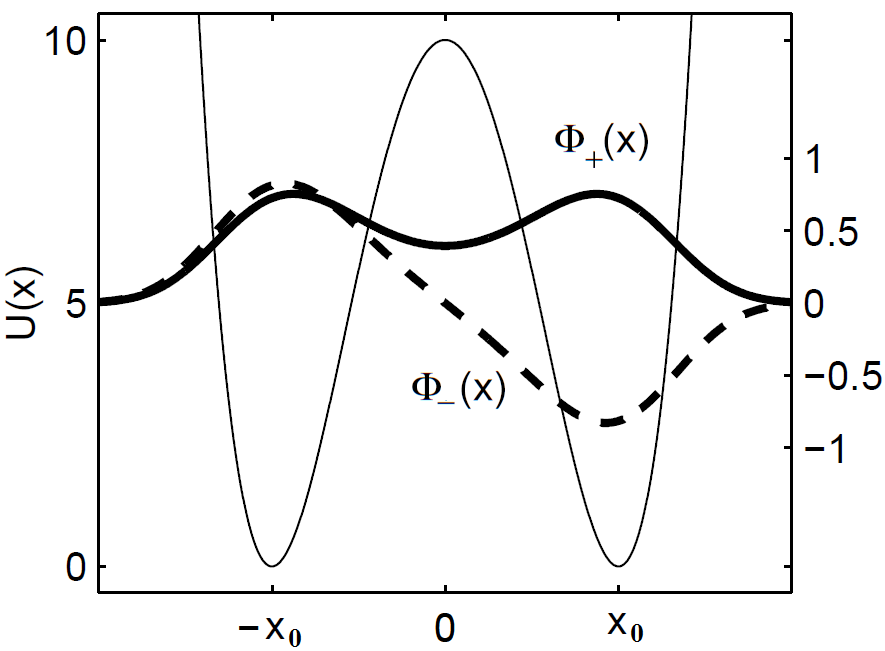
\includegraphics[width=0.5\linewidth]{pic/potential_sym_asym.png}}
%\caption{
%Confined double-well potential for exciton polariton coupled condensate channels with symmetric $(\Phi_+(x))$ and asymmetric $(\Phi_-(x))$ wavefunctions obtained numerically by solving stationary GPE (\ref{eq:stationary}).
%The dimensionless parameters for the calculations are: $h = 10$, $x_0 = 1$, $\mu_+ = 5.7355$, $\mu_- = 6.5653$.
%\label{pic:potential_sym_asym}
%\end{figure}
%
The Hamiltonian for the system of weakly interacting exciton polaritons trapped in an external potential $U(x)$ can be written in the second quantized form as:
%
\begin{equation}
\hat{H} = \int \hat{\psi}^\dag\Big\{ -\dfrac{\hbar^2}{2m_{pol}}  \dfrac{d^2 }{dx^2} + U(x) + \dfrac{g}{2} \hat{\psi}^{\dag} \hat{\psi}  \Big\}\hat{\psi} dx,
\label{eq:gpe_hamiltonian}
\end{equation}
%
where $\hat{\psi} \equiv \hat{\psi}(x, t)$ is a polariton field operator that annihilate a particle at the position $x$ and time $t$, $g$ describes two-body (polariton-polariton) scattering length, $m_{pol}$ is low branch polariton effective mass.
In the paper we use so-called two-mode representation of $\hat{\psi}$ - operator supposing
%
\begin{equation}
\hat{\psi} = \hat{\psi}_1(t) \Phi_1(x) + \hat{\psi}_2(t) \Phi_2(x),
\label{eq:two_modes}
\end{equation}
%
where $\hat{\psi}_{1,2}$ are time dependent operators characterizing condensate at the left and at the right wells respectively; $\Phi_{1,2}(x)$ are condensate wavefunctions which are responsible for it spatial distribution.
It's instructive to represent  $\Phi_{1,2}(x)$ as
%
\begin{equation}
\Phi_{1,2} = \dfrac{\Phi_+ \pm \Phi_-}{\sqrt{2}}
\label{eq:basic_modes}
\end{equation}
%
where $\Phi_{\pm}(x) = \pm \Phi_{\pm}(-x)$ are symmetric ($\Phi_+$) and antisymmetric ($\Phi_-$) real wavefunctions obeying stationary Gross-Pitaevskii (GP) equations $\mu_{\pm} \Phi_{\pm} = -\dfrac{\hbar^2}{2m_{pol}} \dfrac{d^2 \Phi_{\pm}}{dx^2} + U(x) \Phi_{\pm} + g \Phi_{\pm}^3$
%
%\begin{equation}
%\mu_{\pm} \Phi_{\m} = -\dfrac{\hbar^2}{2m} \dfrac{d^2 \Phi_{\pm}}{dx^2} + U(x) \Phi_{\pm} + g \Phi_{\pm}^3.
%\label{eq:stationary}
%\end{equation}
%
and normalization condition $\int \Phi_{\pm}^2 dx = 1$; $\mu_{\pm}$ is chemical potential.
As a result an operator $N=\hat{\psi_1}^\dag\hat{\psi_1} + \hat{\psi_2}^\dag\hat{\psi_2}$ characterizes total number of particles.
Substituting (\ref{eq:basic_modes}), (\ref{eq:two_modes}) into (\ref{eq:gpe_hamiltonian}) we arrive to
% 
\begin{equation}
\begin{array}{lcl}
\hat{H} & = & \dfrac{A}{2} (\hat{\psi}_1^{\dag 2} \hat{\psi}_1^2 + \hat{\psi}_2^{\dag 2} \hat{\psi}_2^2) - \dfrac{G}{2} (\hat{\psi}_1^\dag \hat{\psi}_2 + \hat{\psi}_1 \hat{\psi}_2^\dag) \\ [8pt]
& & -\dfrac{\Gamma}{2} (\hat{\psi}_1^{\dag 2} \hat{\psi}_1 \hat{\psi}_2 + \hat{\psi}_1^\dag \hat{\psi}_1^2 \hat{\psi}_2^\dag + \hat{\psi}_1^\dag \hat{\psi}_2^\dag \hat{\psi}_2^2 + \hat{\psi}_1 \hat{\psi}_2^{\dag 2} \hat{\psi}_2) \\ [8pt]
& & +\dfrac{C}{2} (\hat{\psi}_1^{\dag 2} \hat{\psi}_2^2 + 4 \hat{\psi}_1^\dag \hat{\psi}_1 \hat{\psi}_2^\dag \hat{\psi}_2 + \hat{\psi}_1^2 \hat{\psi}_2^{\dag 2}),
\end{array}
\label{eq:hamiltonian}
\end{equation}
%
where we made denotations $\gamma_{ij} = g \int \Phi_i^2 \Phi_j^2 dx, i,j \in \{+,-\}$,
$A = \frac{1}{4} (\gamma_{++} + \gamma_{--} + 6 \gamma_{+-})$, $\Gamma = \frac{1}{2} (\gamma_{--} - \gamma_{++})$, $C = \frac{1}{4} (\gamma_{++} + \gamma_{--} - 2\gamma_{+-})$, $G = \mu_- - \mu_+ - 2\Gamma$.

Hamiltonian (\ref{eq:hamiltonian}) represents extended model for internal Josephson junction effect with exciton polariton condensates trapped in double-well potential.
The ``additional'' terms with $\Gamma$ and $C$ in (\ref{eq:hamiltonian}) characterize density induced and pair tunneling, respectively.
Generally, our model implies existence of quantum tunneling of the particles between wells with effective (nonlinear) tunneling rate $G_{eff} = \dfrac{1}{2}(G+\Gamma N - C\hat{\psi}_1^\dag\hat{\psi}_2)$.

The contribution from relevant coefficients on can be estimated from variational ansatz $\Phi_{\pm} = A_{\pm} \Big[ \exp \Big( -\dfrac{(x - x_0)^2}{2 a^2} \Big) \pm \exp \Big( -\dfrac{(x + x_0)^2}{2 a^2} \Big) \Big]$, 
%
%\begin{equation}
%\Phi_{\pm} = A_{\pm} \Big[ \exp \Big( -\dfrac{(x - x_0)^2}{2 a^2} \Big) \pm \exp \Big( -\dfrac{(x + x_0)^2}{2 a^2} \Big) \Big],
%\label{eq:two_modes_eq}
%\end{equation}
%
where $a$ is width of condensate wavefunctions at each wells (we suppose them equal to each other), defined from normalization conditions.
% In Fig. \ref{pic:gamma_pm_vs_g} the behavior of normalized coefficients $\dfrac{\gamma_{ij}}{g}$ $i,j \in \{+,-\}$ as a function of half of inter-well distance $x_0$ is shown.
It is important that differences between various $\gamma_{ij}$ rapidly vanish with increasing the inter-well distance $2x_0$.
We can suppose $\Gamma = C = 0$ for $x_0 >> a$.
This limit exactly corresponds to familiar problem of two weakly linked condensates at zero temperature, see e.g. \cite{Aleiner, Shelykh_2008, Borgh_2010, Raghavan}.
%
%\begin{figure}[ht]
%\center{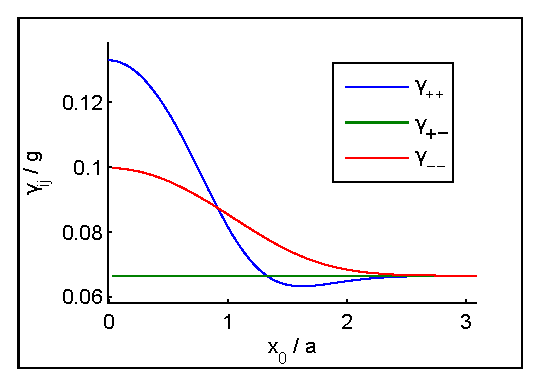
\includegraphics[width=0.5\linewidth]{pic/ypm_x0.eps}}
%\caption{Dependences of normalized matrix elements $\gamma_{ij} / g$ on $x_0 / a$. \label{pic:gamma_pm_vs_g}}
%\end{figure}
%
Now let us introduce the pseudo spin operators
%
\begin{subequations}
\begin{align}
\hat{S}_x = & \dfrac{1}{2} (\hat{\psi}_1^\dag \hat{\psi}_2 + \hat{\psi}_1 \hat{\psi}_2^\dag) \\
\quad \hat{S}_y = & \dfrac{i}{2} (\hat{\psi}_1^\dag \hat{\psi}_2 - \hat{\psi}_1 \hat{\psi}_2^\dag) \\
\hat{S}_z = & \dfrac{1}{2} (\hat{\psi}_2^\dag \hat{\psi}_2 - \hat{\psi}_1^\dag \hat{\psi}_1).
\end{align}
\label{eq:pseudo_spin}
\end{subequations}
%
Inserting (\ref{eq:pseudo_spin}) into the (\ref{eq:hamiltonian}) we arrive at Eq.(1)  
with 
%the equation
%
%\begin{equation}
%\hat{H} = \alpha \hat{S}_z^2 + \beta %\hat{S}_x^2 - B \hat{S}_x,
%\label{eq:hamiltonain_spin_appendix}
%\end{equation}
%
$\alpha = A - C = 2\gamma_{\pm} > 0$, $\beta = 2C > 0$ and $B = \Gamma N + G > 0$.
We also chose $x_0$ obeying the condition $\gamma_{++} \simeq \gamma_{--} = \gamma$ supposing $\Gamma = 0$ for simplicity.

% Create the reference section using BibTeX:
\bibliography{list}

\end{document}